

\chapter{Metodologia}

\section{Componentes}

\subsection{Motor DC e driver}
Optou-se pelo uso de um motor DC de 6V 210rpm, com taxa de redução de 1:34. O motor já possiu um encoder magnético acoplado, com 11 PPR (\textit{Pulses Per Revolution}).
Será usado o driver Ponte H L298N para uso incial, suporta até 2A em operação DC \cite{datasheel_l298n}, a corrente de operação máxima do motor é de 1.1A, 
porém a corrente de parada é drenar 3.2A.
O L298N também causa uma queda de tensão, a 1A pode causar uma queda de 3.2V, fazendo com que o motor não receba a tensão necessária para operar nos valores desejados \cite{datasheel_l298n},
Com isso, um driver de maior capacidade possa ser necessário, as opções são os da categoria \textit{Medium-power} da Pololu, DRV8874 ou acima \cite{DRV8874}.
Mas para seguir com desenvolvimento, o l298N será usado por hora.

\begin{figure}[h]
	\centering
	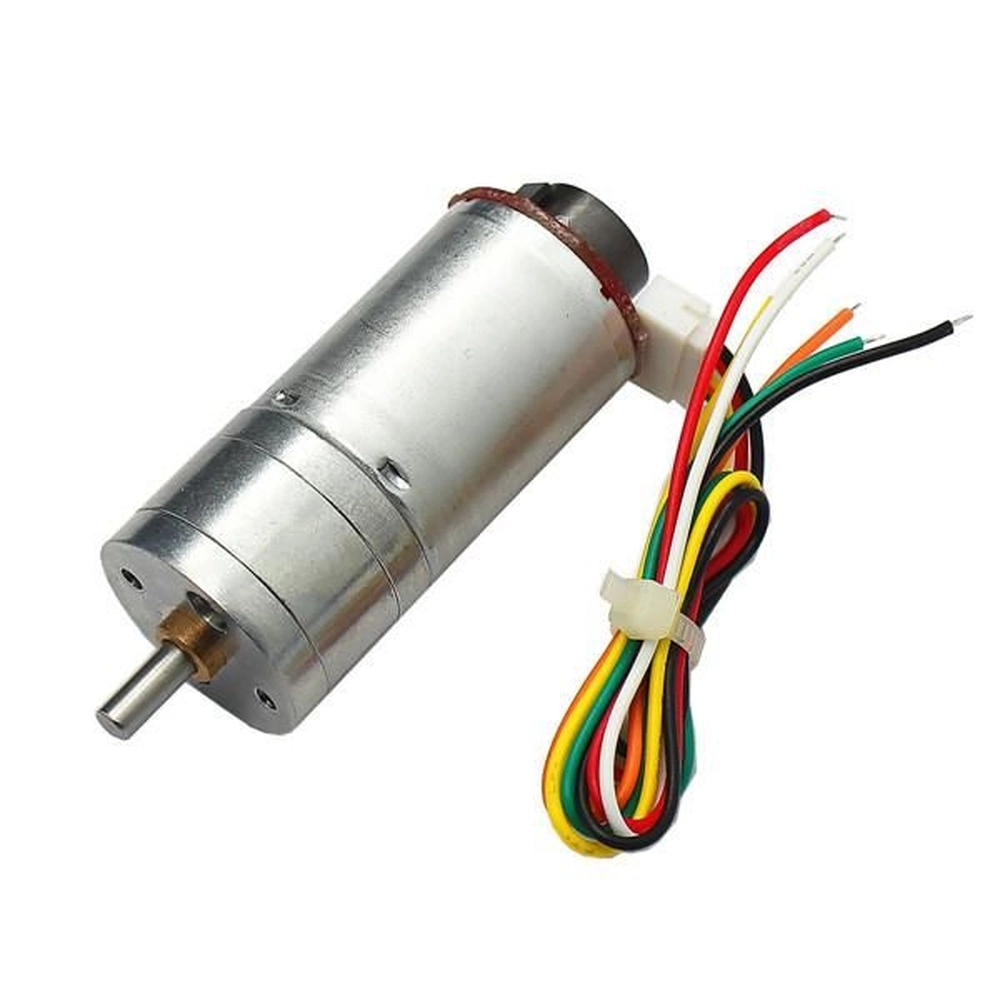
\includegraphics[width=0.7\textwidth]{figures/CHR_GM25_370}
	\caption{Motor DC 6V \cite{motor_dc_6v_encoder}}
\end{figure}


\begin{quadro}[htb]
	\caption{\label{Especificacoes_motordc_6v}Especificações do motor DC 6V}
	 \begin{tabular}{|c|c|c|c|}
		\hline
		\textbf{Componente} & \textbf{Quant} \\ \hline
		Tensão nominal & DC 6V  \\ \hline
		Velocidade sem carga  & 210RPM 0.13A  \\ \hline
		Eficiência máxima & 2,0kg.cm/170rpm/2,0W/0,60A   \\ \hline
		Poder maximo & 5,2kg.cm/110rpm/3,1W/1,10A   \\ \hline
		Torque de parada  & 10kg.cm 3.2A    \\ \hline
		Taxa de Redução do Retardador & 1:34  \\ \hline
		Resolução do salão & Razão Hall x 34,02 = 341,2PPR  \\ \hline
	\end{tabular}
	\fonte{\cite{chinhai_motor}}
	\end{quadro}

\begin{figure}[h]
	\centering
	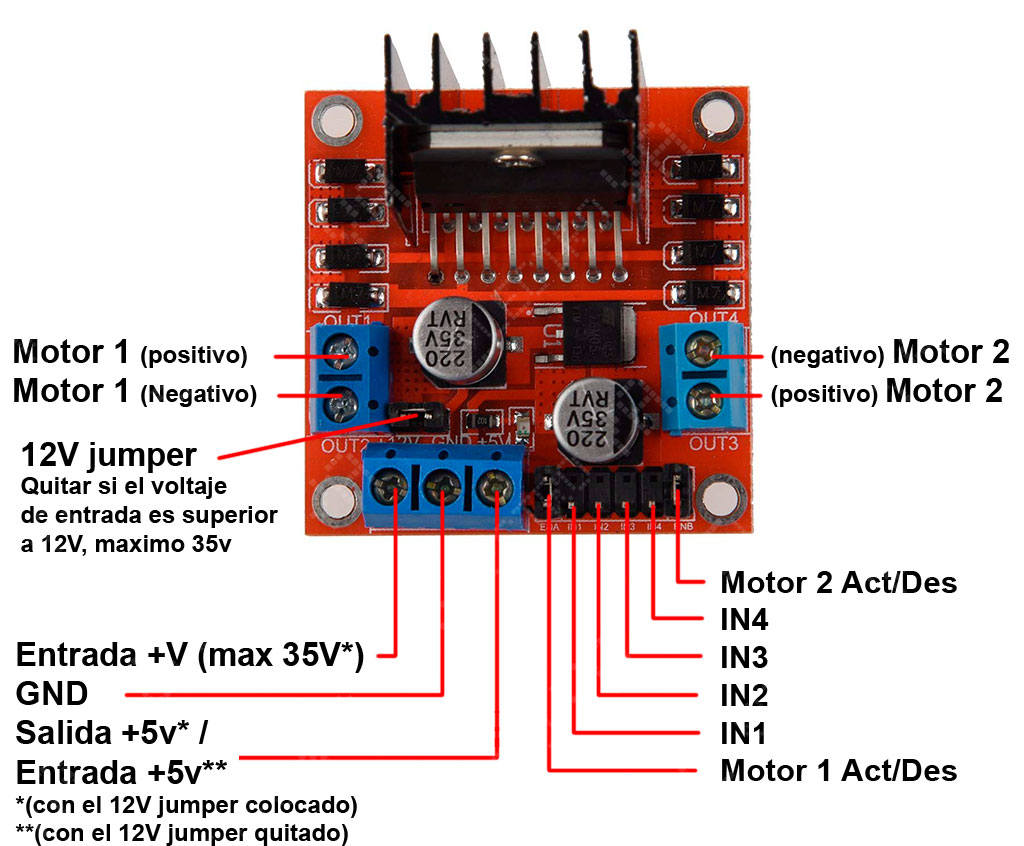
\includegraphics[width=0.7\textwidth]{figures/l289n}
	\caption{Driver Ponte H L289N \cite{l289n}}
\end{figure}

	
\subsection{Microcontrolador}

Para microcontrolador, optou-se pelo uso do  STM32F103C8, também conhecido como Blue Pill.
Possui como processador o ARM Cortex-M3, e tem 64Kbs de memória flash. 
O STM32F103C8 possui 7 timers, 2 ADCs, e 9 interfaces de comunicação, incluindo
I2C (\textit{Inter-Integrated Circuit}), USART (\textit{Universal Synchronous
Asynchronous Receiver Transmitter}), SPI (\textit{Serial Peripheral Interface}),
CAN e USB 2.0.
O STM32F103C8 possui 6 que suportam canais de PWM de 5V, e outros 8 canais de 3.3V,  e pode ser alimentado via micro USB de 5V.

Para carregar o projeto no microcontrolador, um gravador ST-LINK USB será utilizado.

\begin{figure}[h]
	\centering
	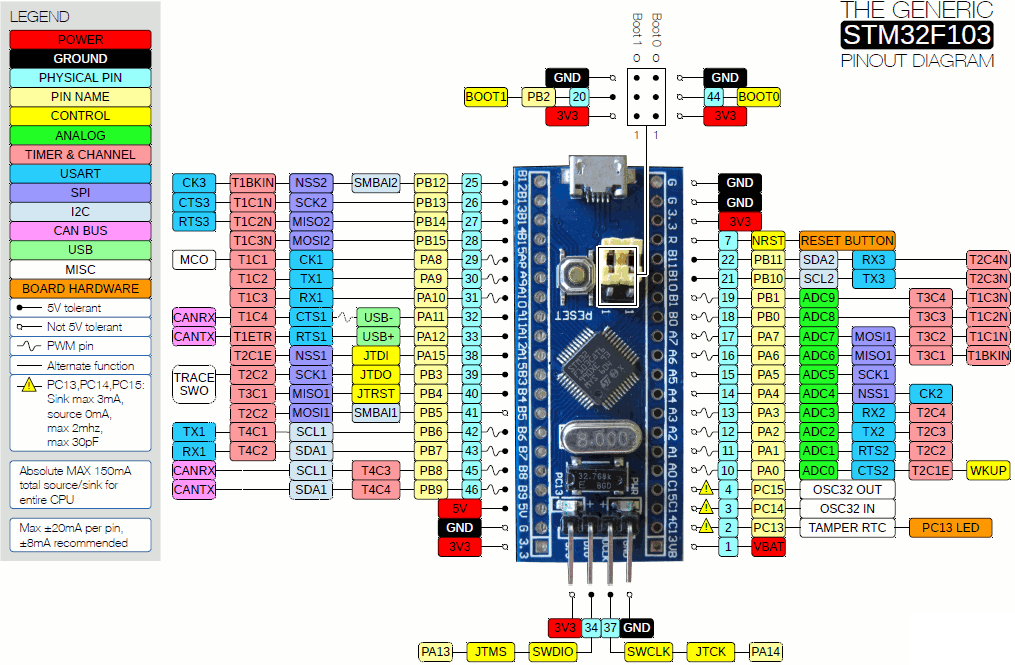
\includegraphics[width=0.8\textwidth]{figures/stm32f1_pinout}
	\caption{Diagrama de pinos do STM32F103C8}
\end{figure}

\subsection{Alimentação}
Para alimentar o microntrolador, um powerbank com saida de 5v será usado, considerando que o STM32F103C8 funciona a uma corrente abaixo de 100mA
Para alimentar os motores, para uso no desenvolvimento, optou-se o uso de pilhas AA (1,5V) e um suporte para 4 pilhas, 
mas será necessário trocar por bateria de lítio-ion.

\subsection{Controle do robô}
Inicialmente será usado um joystick de 3 eixos para controlar o robô para testar a cinemática de movimento.

\subsection{Desenvolvimento do código do projeto}
O projeto será codado em C, usando a IDE Atollic TrueSTUDIO.
O código deverá conter o controle do PWM para os motores, e controle da cinemática.
